\section{Tartószerkezet és 3D nyomtatott váz}

A drónok tervezése és építése során az egyik legfontosabb szempont a stabil és megbízható tartószerkezet kialakítása. Az alkalmazott anyagok és technológiák döntően befolyásolják a drón repülési jellemzőit, terhelhetőségét és élettartamát. A projektünk során a 3D nyomtatási technológiát választottuk a váz és a tartószerkezet létrehozásához, mivel ez a módszer számos előnyt kínál a hagyományos gyártási technikákkal szemben.

Az alkalmazott 3D nyomtatási technológia lehetővé teszi a komplex geometriák és precíz részletek létrehozását, amelyek különösen fontosak a drón szerkezetének optimalizálása és a súlycsökkentés szempontjából. A 3D nyomtatott váz könnyű, mégis rendkívül erős, ami hozzájárul a drón stabil repülési tulajdonságaihoz és hosszú élettartamához.

A drón vázát 70\%-os kitöltéssel nyomtattuk PET-G anyagból, amely erős és ellenálló, miközben megőrzi a szükséges rugalmasságot és könnyűséget. Az egyes aklatrészek rögzítése egymáshoz 16 darab M5-ös 20 miliméteres hexagon fejű csavarral és M5-ös anyával történt. 

\begin{figure}[H]
	\centering
	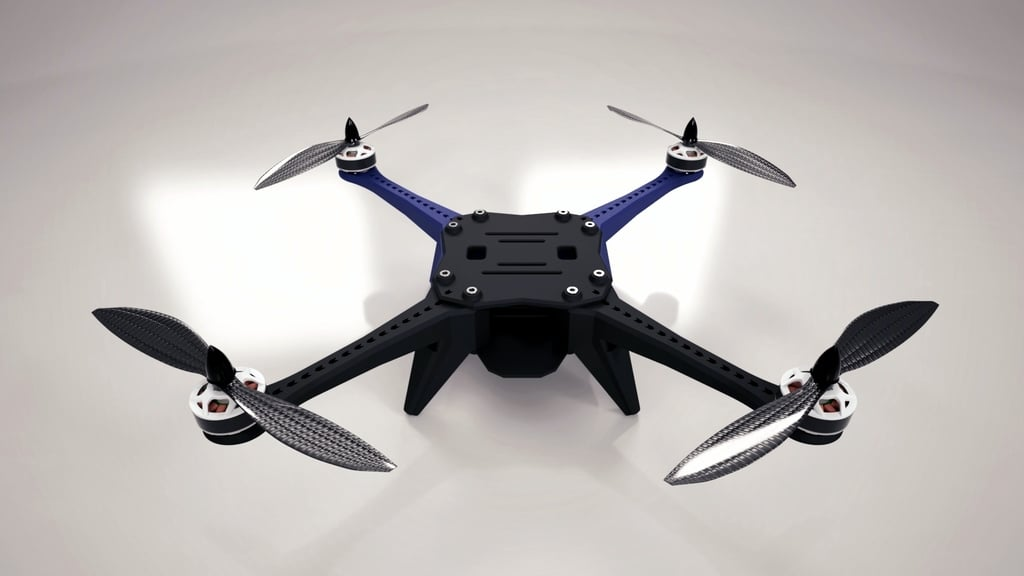
\includegraphics[scale=0.3]{figures/drone_model.JPG}
	\caption{A drón 3D -s modellje}
	\label{A drón 3D -s modellje}
\end{figure}

\section{Elektronikai aklatrészek}

Az alábbiakban a drón motorjairól, elektronikus fordulatszám-szabályozóiról (ESC), az akkumulátorról, valamint a központi vezérlőegységről esik szó.

\subsection{BLDC motorok}
A drón meghajtását négy darab kefe nélküli egyenáramú (Brushless DC, BLDC) motor biztosítja. Ezek a motorok a magas hatékonyságuk és tartósságuk miatt ideálisak drónokhoz. A kefe nélküli kialakítás előnye, hogy minimalizálja a mechanikai kopást, így hosszabb élettartamot és kevesebb karbantartást igényel.

A motorok forgómágneses rendszere és a szállítólégcsavarok (propellerek) közvetlenül a drón stabilitásáért felelősek. A négy motor együttműködése lehetővé teszi a drón emelkedését, süllyedését, valamint forgását és előre-hátra irányuló mozgását.


\begin{figure}[H]
	\centering
	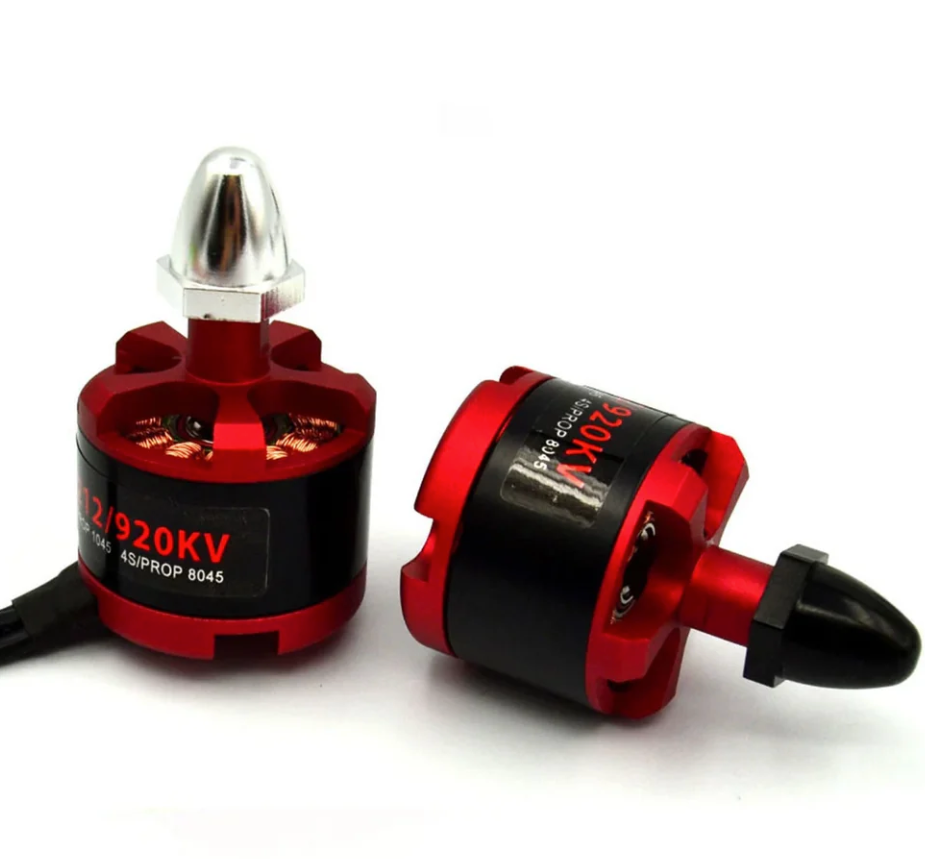
\includegraphics[scale=0.3]{bldc_motor.png}
	\caption{Drónhoz felhasznált BLDC motrok}
	\label{Drónhoz felhasznált BLDC motrok}
\end{figure}

\subsection{ESC-k}
A motorok működését négy elektronikus fordulatszám-szabályozó (Electronic Speed Controller, ESC) vezérli. Az ESC-k feladata, hogy az akkumulátorból érkező elektromos energiát a motorok számára megfelelő frekvenciájú és amplitódójú jelré alakítsák. Ezáltal az ESC-k precíz szabályozást biztosítanak a motorok forgási sebességéhez, ami kulcsfontosságú a drón stabilitása és irányíthatósága szempontjából.

Az általam használt ESC-k beépített védelmi mechanizmusokkal rendelkeznek, amelyek megakadályozzák a túlmelegedést és a túláram miatti meghibásokat. Továbbá, ezek a szabályozók kompatibilisek a BLDC motorokkal, ami garantálja a rendszer zavartalan működését.

\begin{figure}[H]
	\centering
	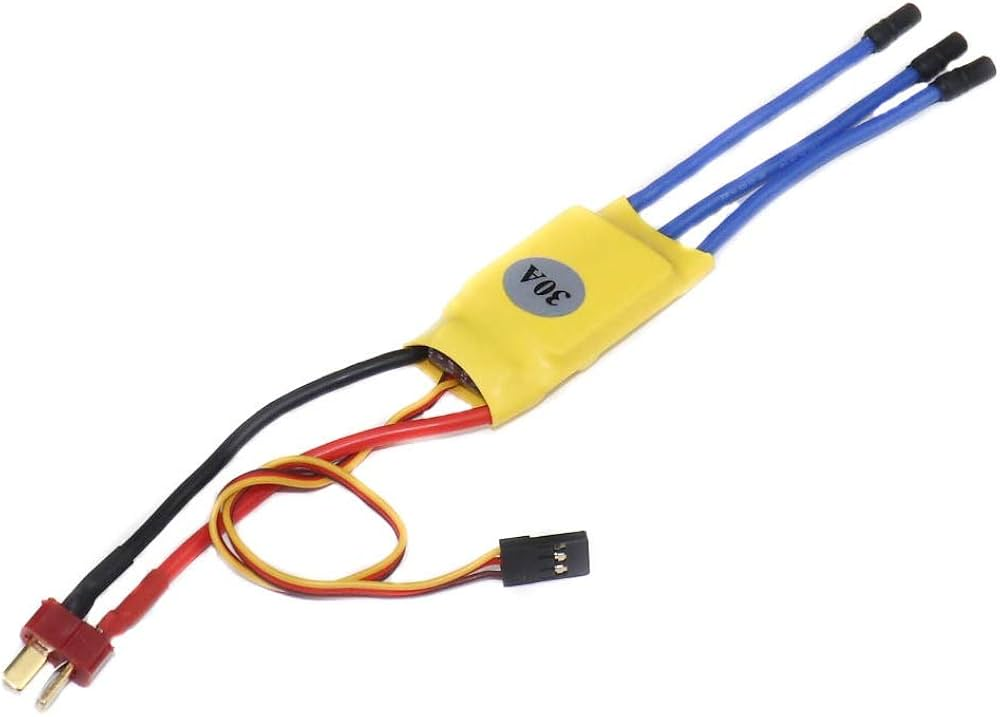
\includegraphics[scale=0.3]{esc.jpg}
	\caption{Drónhoz felhasznált ESC-k}
	\label{Drónhoz felhasznált ESC-k}
\end{figure}

\subsection{Akkumulátor}
A drón energiaellátását egy nagy kapacitású lítium-polimer (LiPo) akkumulátor biztosíthatja. Az akkumulátor kiválasztásakor figyelembe kell venni a drón súlyát, a motorok áramfogyasztását és a kívánt repülési időt. A LiPo akkumulátorok előnye, hogy magas energiasűrűséggel rendelkeznek, ami lehetővé teszi a hosszabb repülési időt anélkül, hogy jelentős súlyt adnának a drónhoz.

\begin{figure}[H]
	\centering
	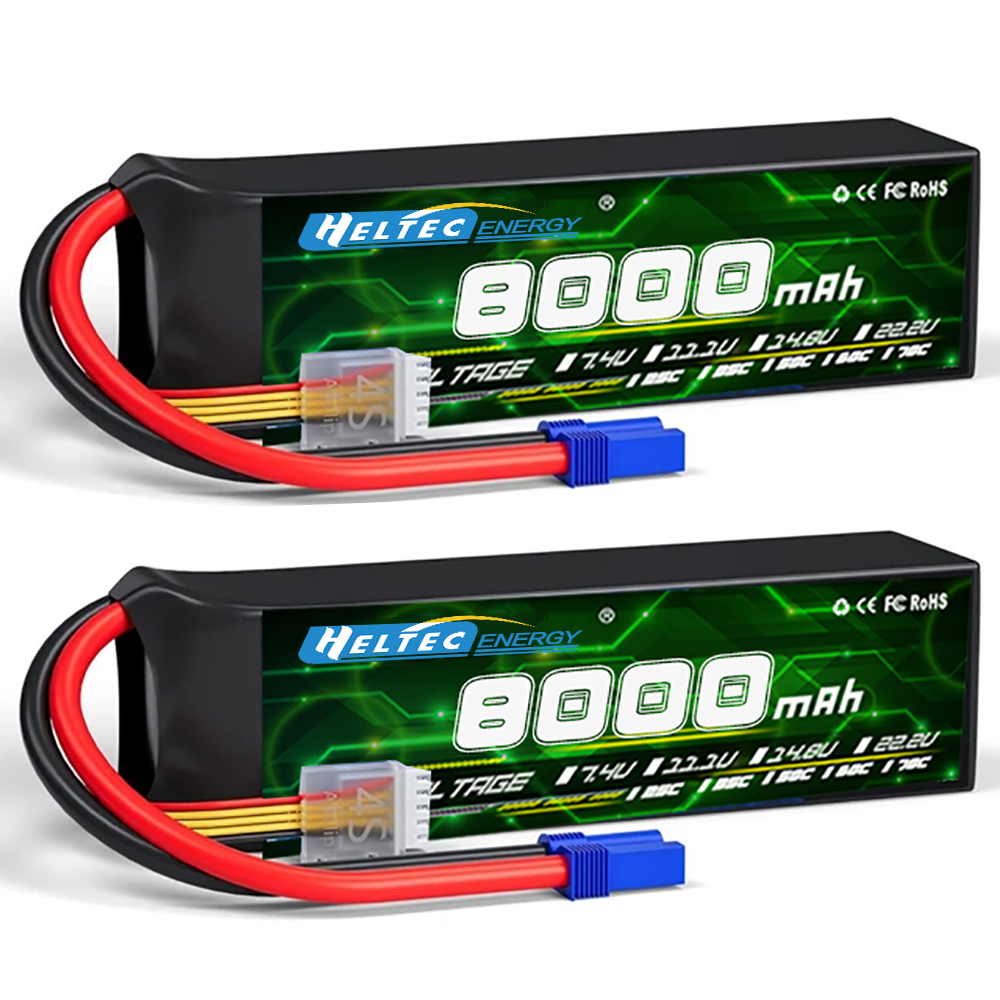
\includegraphics[scale=0.25]{battery.jpg}
	\caption{Drónhoz felhasználható akkumulátorok}
	\label{Drónhoz felhasznált ESC-kDrónhoz felhasználható akkumulátorok}
\end{figure}

\subsection{Központi vezérlőegység}
A drón "agya" a központi vezérlőegység, amely a rendszer minden elemét összehangolja. 

Ez a vezérlőegység tartalmazza a drón stabilitását biztosító algoritmusokat, így mint a PID szabályozást, amely minimalizálja a lengéseket és stabilizálja a drónt repülés közben. Továbbá, a vezérlőegység kapcsolódik a távirányítóhoz és a GPS modulhoz, ami lehetővé teszi az automatikus és manuális repülési módok közötti váltást.

\subsubsection{IMU (Inerciális mérőegység)}
Az IMU (Inertial Measurement Unit) egy kulcsfontosságú szenzor, amely a drón mozgásának és orientációjának pontos mérését végzi. Az IMU tipikusan gyorsulásmérőket (accelerometer), giroszkópokat (gyroscope) és néha magnetométereket is tartalmaz, amelyek segítségével az alábbi adatokat méri:

Lineáris gyorsulás: A drón mozgási sebességének változása az x, y és z tengelyek mentén.

Szögsebesség: A drón forgási sebessége a giroszkóp adatai alapján, amely a roll, pitch és yaw tengelyeken történő forgást méri.

Mágneses mező iránya: A magnetométer segítségével meghatározható a drón relatív iránya a Föld mágneses teréhez képest.

Az IMU által mért adatok valós időben kerülnek feldolgozásra a központi vezérlőegységben. Ezek az adatok nélkülözhetetlenek a drón stabilitásának fenntartásához és pontos irányításához. A vezérlőegység a kapott értékeket folyamatosan elemzi, és szükség esetén korrigálja a motorok sebességét a megfelelő stabilitás és iránytartás érdekében.

A gyorsulásmérő adatai segítenek a drón helyzetének meghatározásában, míg a giroszkóp adatai a forgás stabilizálásában játszanak szerepet. A magnetométer, ha rendelkezésre áll, további pontosságot biztosít az iránymeghatározásban, különösen akkor, ha a drón GPS-alapú navigációt végez.

Az IMU által szolgáltatott pontos és gyors adatok lehetővé teszik, hogy a drón dinamikusan alkalmazkodjon a környezeti változásokhoz, például szélmozgáshoz vagy hirtelen irányváltásokhoz, biztosítva ezzel a megbízható és zökkenőmentes repülést.

\subsubsection{Kalman-szűrő}
A Kalman-szűrő egy matematikai algoritmus, amelyet a drón vezérlőegysége használ az IMU és más szenzorok által szolgáltatott adatok pontosítására és zajcsökkentésére. Ez az algoritmus különösen fontos a drón repülési stabilitásának és irányításának biztosításához, mivel a szenzorok adatai gyakran zajosak és pontatlanok lehetnek.

A Kalman-szűrő az alábbi lépéseket hajtja végre:

Előrejelzés: A rendszer aktuális állapotából (például pozíció, sebesség, orientáció) előrejelzi a következő állapotot egy dinamikai modell alapján.

Mérés: Az IMU és más szenzorok új adatokat szolgáltatnak az aktuális állapotról.

Frissítés: Az előrejelzett állapotot összehasonlítja a mért adatokkal, és korrigálja az előrejelzést, figyelembe véve a szenzorok pontosságát és a mérési zajt.

A Kalman-szűrő alkalmazásával a drón vezérlőegysége képes pontosabb állapotbecslésre, amely alapját képezi a stabil repülésnek és a precíz irányításnak. Például, ha az IMU giroszkópja és gyorsulásmérője kissé eltérő adatokat ad, a Kalman-szűrő a két forrás kombinációjával egy pontosabb képet nyújt a drón valódi mozgásáról.

Ez az algoritmus kulcsfontosságú a dinamikus környezetekben, ahol a drónnak gyorsan és pontosan kell reagálnia a külső hatásokra, például szélre vagy akadályokra. A Kalman-szűrő alkalmazása jelentősen javítja a rendszer megbízhatóságát és teljesítményét, különösen az autonóm repülési funkciók esetében.